\documentclass[9pt]{ctexart}
\usepackage[utf8]{inputenc}
\usepackage[left=0.4in,right=0.4in,top=0.7in,bottom=0.4in]{geometry}
\usepackage{fancyhdr}
\usepackage{amsmath}
\usepackage{amssymb}
\usepackage{multicol}
\usepackage{ctex}
\usepackage{graphicx}
\usepackage{pdflscape}

\usepackage{titlesec}
\titlespacing\section{0pt}{12pt}{0pt}
\titlespacing\subsection{0pt}{5pt}{0pt}
\titlespacing\subsubsection{0pt}{5pt}{0pt}

\usepackage{enumitem}
\setlist{nolistsep}

\pagestyle{fancy}
\fancyhead[L]{East China Normal University}
\fancyhead[R]{\thepage}
\fancyfoot[C]{}

\fancypagestyle{plain}
{
\fancyhead[L]{East China Normal University}
\fancyhead[R]{\thepage}
\fancyfoot[C]{}
}

\setcounter{page}{22}

\begin{document}
\begin{landscape}

\begin{multicols}{2}

\section{数学}

\subsection{杜教筛}

求 $S(n)=\sum_{i=1}^n f(i)$,其中 $f$ 是一个积性函数。

构造一个积性函数 $g$,那么由 $(f*g)(n)=\sum_{d|n}f(d)g(\frac{n}{d})$,得到 $f(n)=(f*g)(n)-\sum_{d|n,d<n}f(d)g(\frac{n}{d})$。

\begin{eqnarray}
g(1)S(n)&=&\sum_{i=1}^n (f*g)(i)-\sum_{i= 1}^{n}\sum_{d|i,d<i}f(d)g(\frac{n}{d}) \\
&\overset{t=\frac{i}{d}}{=}& \sum_{i=1}^n (f*g)(i)-\sum_{t=2}^{n} g(t) S(\lfloor \frac{n}{t} \rfloor)
\end{eqnarray}

当然,要能够由此计算 $S(n)$,会对 $f,g$ 提出一些要求:

\begin{itemize}
\item $f*g$ 要能够快速求前缀和。
\item $g$  要能够快速求分段和(前缀和)。
\item 对于正常的积性函数 $g(1)=1$,所以不会有什么问题。
\end{itemize}

在预处理 $S(n)$ 前 $n^{\frac{2}{3}}$ 项的情况下复杂度是 $O(n^{\frac{2}{3}})$。

\subsection{素性测试}

\begin{itemize}
    \item 前置:快速乘、快速幂
    \item int 范围内只需检查 2, 7, 61
    \item long long 范围 2, 325, 9375, 28178, 450775, 9780504, 1795265022
    \item 3E15 内 2, 2570940, 880937, 610386380, 4130785767
    \item 4E13 内 2, 2570940, 211991001, 3749873356
    \item http://miller-rabin.appspot.com/
\end{itemize}

\subsection{扩展欧几里得}

\begin{itemize}
\item 求 $ax+by=gcd(a,b)$ 的一组解
\item 如果 $a$ 和 $b$ 互素,那么 $x$ 是 $a$ 在模 $b$ 下的逆元
\item 注意 $x$ 和 $y$ 可能是负数
\end{itemize}

\subsection{类欧几里得}
\begin{itemize}
\item $m = \lfloor \frac{an+b}{c} \rfloor$.
\item $f(a,b,c,n)=\sum_{i=0}^n\lfloor\frac{ai+b}{c}\rfloor$: 当 $a \ge c$ or $b \ge c$ 时,$f(a,b,c,n)=(\frac{a}{c})n(n+1)/2+(\frac{b}{c})(n+1)+f(a \bmod c,b \bmod c,c,n)$;否则 $f(a,b,c,n)=nm-f(c,c-b-1,a,m-1)$。
\item $g(a,b,c,n)=\sum_{i=0}^n i \lfloor\frac{ai+b}{c}\rfloor$: 当 $a \ge c$ or $b \ge c$ 时,$g(a,b,c,n)=(\frac{a}{c})n(n+1)(2n+1)/6+(\frac{b}{c})n(n+1)/2+g(a \bmod c,b \bmod c,c,n)$;否则 $g(a,b,c,n)=\frac{1}{2} (n(n+1)m-f(c,c-b-1,a,m-1)-h(c,c-b-1,a,m-1))$。
\item $h(a,b,c,n)=\sum_{i=0}^n\lfloor \frac{ai+b}{c} \rfloor^2$: 当 $a \ge c$ or $b \ge c$ 时,$h(a,b,c,n)=(\frac{a}{c})^2 n(n+1)(2n+1)/6 +(\frac{b}{c})^2 (n+1)+(\frac{a}{c})(\frac{b}{c})n(n+1)+h(a \bmod c, b \bmod c,c,n)+2(\frac{a}{c})g(a \bmod c,b \bmod c,c,n)+2(\frac{b}{c})f(a \bmod c,b \bmod c,c,n)$;否则 $h(a,b,c,n)=nm(m+1)-2g(c,c-b-1,a,m-1)-2f(c,c-b-1,a,m-1)-f(a,b,c,n)$。
\end{itemize}

\subsection{斯特灵数}
\begin{itemize}
\item 第一类斯特灵数:绝对值是 $n$ 个元素划分为 $k$ 个环排列的方案数。$s(n,k)=s(n-1,k-1)+(n-1)s(n-1,k)$
\item 第二类斯特灵数:$n$ 个元素划分为 $k$ 个等价类的方案数。 $S(n, k)=S(n-1,k-1)+kS(n-1, k)$
\end{itemize}


\subsection{一些数论公式}

\begin{itemize}
  \item 当 $x\geq\phi(p)$ 时有 $a^x\equiv a^{x \; mod \; \phi(p) + \phi(p)}\pmod p$
  \item $\mu^2(n)=\sum_{d^2|n} \mu(d)$
  \item $\sum_{d|n} \varphi(d)=n$
  \item $\sum_{d|n} 2^{\omega(d)}=\sigma_0(n^2)$,其中 $\omega$ 是不同素因子个数
  \item $\sum_{d|n} \mu^2(d)=2^{\omega(d)}$
\end{itemize}

\subsection{一些数论函数求和的例子}

\begin{itemize}
  \item $\sum_{i=1}^n i[gcd(i, n)=1] = \frac {n \varphi(n) + [n=1]}{2}$
  \item $\sum_{i=1}^n \sum_{j=1}^m [gcd(i,j)=x]=\sum_d \mu(d) \lfloor \frac n {dx} \rfloor  \lfloor \frac m {dx} \rfloor$
  \item $\sum_{i=1}^n \sum_{j=1}^m gcd(i, j) = \sum_{i=1}^n \sum_{j=1}^m \sum_{d|gcd(i,j)} \varphi(d) = \sum_{d} \varphi(d) \lfloor \frac nd \rfloor \lfloor \frac md \rfloor$
  \item $S(n)=\sum_{i=1}^n \mu(i)=1-\sum_{i=1}^n \sum_{d|i,d < i}\mu(d) \overset{t=\frac id}{=} 1-\sum_{t=2}^nS(\lfloor \frac nt \rfloor)$(利用 $[n=1] = \sum_{d|n} \mu(d)$)
  \item $S(n)=\sum_{i=1}^n \varphi(i)=\sum_{i=1}^n i-\sum_{i=1}^n \sum_{d|i,d<i} \varphi(i)\overset{t=\frac id}{=} \frac {i(i+1)}{2} - \sum_{t=2}^n S(\frac n t)$(利用 $n = \sum_{d|n} \varphi(d)$)
  \item $\sum_{i=1}^n \mu^2(i) = \sum_{i=1}^n \sum_{d^2|n} \mu(d)=\sum_{d=1}^{\lfloor \sqrt n \rfloor}\mu(d) \lfloor \frac n {d^2} \rfloor$ 
  \item $\sum_{i=1}^n \sum_{j=1}^n gcd^2(i, j)= \sum_{d} d^2 \sum_{t} \mu(t) \lfloor \frac n{dt} \rfloor ^2 \\
  \overset{x=dt}{=} \sum_{x} \lfloor \frac nx \rfloor ^ 2 \sum_{d|x} d^2 \mu(\frac tx)$
  \item $\sum_{i=1}^n \varphi(i)=\frac 12 \sum_{i=1}^n \sum_{j=1}^n [i \perp j] - 1=\frac 12 \sum_{i=1}^n \mu(i) \cdot\lfloor \frac n i \rfloor ^2-1$
\end{itemize}

\subsection{斐波那契数列性质}

\begin{itemize}
  \item $F_{a+b}=F_{a-1} \cdot F_b+F_a \cdot F_{b+1}$
  \item $F_1+F_3+\dots +F_{2n-1} = F_{2n},F_2 + F_4 + \dots + F_{2n} = F_{2n + 1} - 1$
  \item $\sum_{i=1}^n F_i = F_{n+2} - 1$
  \item $\sum_{i=1}^n F_i^2 = F_n \cdot F_{n+1}$
  \item $F_n^2=(-1)^{n-1} + F_{n-1} \cdot F_{n+1}$
  \item $gcd(F_a, F_b)=F_{gcd(a, b)}$
  \item 模 $n$ 周期(皮萨诺周期)
  \begin{itemize}
    \item $\pi(p^k) = p^{k-1} \pi(p)$
    \item $\pi(nm) = lcm(\pi(n), \pi(m)), \forall n \perp m$
    \item $\pi(2)=3, \pi(5)=20$
    \item $\forall p \equiv \pm 1\pmod {10}, \pi(p)|p-1$
    \item $\forall p \equiv \pm 2\pmod {5}, \pi(p)|2p+2$
  \end{itemize}
\end{itemize}

\subsection{常见生成函数}

\begin{itemize}
  \item $(1+ax)^n=\sum_{k=0}^n \binom {n}{k} a^kx^k$
  \item $\dfrac{1-x^{r+1}}{1-x}=\sum_{k=0}^nx^k$
  \item $\dfrac1{1-ax}=\sum_{k=0}^{\infty}a^kx^k$
  \item $\dfrac 1{(1-x)^2}=\sum_{k=0}^{\infty}(k+1)x^k$
  \item $\dfrac1{(1-x)^n}=\sum_{k=0}^{\infty} \binom{n+k-1}{k}x^k$
  \item $e^x=\sum_{k=0}^{\infty}\dfrac{x^k}{k!}$
  \item $\ln(1+x)=\sum_{k=0}^{\infty}\dfrac{(-1)^{k+1}}{k}x^k$
\end{itemize}

\subsection{佩尔方程}

若一个丢番图方程具有以下的形式:$x^2 - ny^2= 1$。且 $n$ 为正整数,则称此二元二次不定方程为\textbf{佩尔方程}。

若 $n$ 是完全平方数,则这个方程式只有平凡解 $(\pm 1,0)$(实际上对任意的 $n$,$(\pm 1,0)$ 都是解)。对于其余情况,拉格朗日证明了佩尔方程总有非平凡解。而这些解可由 $\sqrt{n}$ 的连分数求出。

$x = [a_0; a_1, a_2, a_3]=x = a_0 + \cfrac{1}{a_1 + \cfrac{1}{a_2 + \cfrac{1}{a_3 + \cfrac{1}{\ddots\,}}}}$

设 $\tfrac{p_i}{q_i}$ 是 $\sqrt{n}$ 的连分数表示:$[a_{0}; a_{1}, a_{2}, a_{3}, \,\ldots ]$ 的渐近分数列,由连分数理论知存在 $i$ 使得 $(p_i,q_i)$ 为佩尔方程的解。取其中最小的 $i$,将对应的 $(p_i,q_i)$ 称为佩尔方程的基本解,或最小解,记作 $(x_1,y_1)$,则所有的解 $(x_i,y_i)$ 可表示成如下形式:$x_{i}+y_{i}{\sqrt  n}=(x_{1}+y_{1}{\sqrt  n})^{i}$。或者由以下的递回关系式得到:

$\displaystyle x_{i+1} = x_1 x_i + n y_1 y_i$, $\displaystyle y_{{i+1}}=x_{1}y_{i}+y_{1}x_{i}$。

通常,佩尔方程结果的形式通常是 $a_n=ka_{n−1}−a_{n−2}$($a_{n−2}$ 前的系数通常是 $−1$)。暴力 / 凑出两个基础解之后加上一个 $0$,容易解出 $k$ 并验证。

\subsection{Burnside \& Polya}

$|X/G|={\frac  {1}{|G|}}\sum _{{g\in G}}|X^{g}|$。$X^g$ 是 $g$ 下的不动点数量,也就是说有多少种东西用 $g$ 作用之后可以保持不变。

$|Y^X/G| = \frac{1}{|G|}\sum_{g \in G} m^{c(g)}$。用 $m$ 种颜色染色,然后对于某一种置换 $g$,有 $c(g)$ 个置换环,为了保证置换后颜色仍然相同,每个置换环必须染成同色。

\subsection{皮克定理}

$2S = 2a+b-2$

\begin{itemize}
  \item $S$ 多边形面积
  \item $a$ 多边形内部点数
  \item $b$ 多边形边上点数
\end{itemize}

\subsection{莫比乌斯反演}

\begin{itemize}
  \item $g(n) = \sum_{d|n} f(d) \Leftrightarrow f(n) = \sum_{d|n} \mu (d) g( \frac{n}{d})$
  \item $f(n)=\sum_{n|d}g(d) \Leftrightarrow g(n)=\sum_{n|d} \mu(\frac{d}{n}) f(d)$
\end{itemize}

\subsection{低阶等幂求和}

\begin{itemize}
  \item $\sum_{i=1}^{n} i^{1} = \frac{n(n+1)}{2} = \frac{1}{2}n^2 +\frac{1}{2} n$
  \item $\sum_{i=1}^{n} i^{2} = \frac{n(n+1)(2n+1)}{6} = \frac{1}{3}n^3 + \frac{1}{2}n^2 + \frac{1}{6}n$
  \item $\sum_{i=1}^{n} i^{3} = \left[\frac{n(n+1)}{2}\right]^{2} = \frac{1}{4}n^4 + \frac{1}{2}n^3 + \frac{1}{4}n^2$
  \item $\sum_{i=1}^{n} i^{4} = \frac{n(n+1)(2n+1)(3n^2+3n-1)}{30} = \frac{1}{5}n^5 + \frac{1}{2}n^4 + \frac{1}{3}n^3 - \frac{1}{30}n$
  \item $\sum_{i=1}^{n} i^{5} = \frac{n^{2}(n+1)^{2}(2n^2+2n-1)}{12} = \frac{1}{6}n^6 + \frac{1}{2}n^5 + \frac{5}{12}n^4 - \frac{1}{12}n^2$
\end{itemize}

\subsection{一些组合公式}

\begin{itemize}
  \item 错排公式:$D_1=0,D_2=1,D_n=(n-1)(D_{n-1} + D_{n-2})=n!(\frac 1{2!}-\frac 1{3!}+\cdots + (-1)^n\frac 1{n!})=\lfloor \frac{n!}e + 0.5 \rfloor$
  \item 卡塔兰数($n$ 对括号合法方案数,$n$ 个结点二叉树个数,$n\times n$ 方格中对角线下方的单调路径数,凸 $n+2$ 边形的三角形划分数,$n$ 个元素的合法出栈序列数):$C_n=\frac 1{n+1} \binom {2n}{n}=\frac{(2n)!}{(n+1)!n!}$
\end{itemize}

\subsection{伯努利数与等幂求和}

$\sum_{i=0}^n i^k = \frac{1}{k+1} \sum_{i=0}^k \binom{k+1}{i} B_{k+1-i} (n+1)^i$。也可以 $\sum_{i=0}^n i^k = \frac{1}{k+1} \sum_{i=0}^k \binom{k+1}{i} B^+_{k+1-i} n^i$。区别在于 $B^+_1 =1/2$。

\subsection{数论分块}

$f(i) = \lfloor \frac{n}{i} \rfloor=v$ 时 $i$ 的取值范围是 $[l,r]$。

\begin{verbatim}
for (LL l = 1, v, r; l <= N; l = r + 1) {
    v = N / l; r = N / v;
}
\end{verbatim}

\subsection{博弈}

\begin{itemize}
\item Nim 游戏:每轮从若干堆石子中的一堆取走若干颗。先手必胜条件为石子数量异或和非零。
\item 阶梯 Nim 游戏:可以选择阶梯上某一堆中的若干颗向下推动一级,直到全部推下去。先手必胜条件是奇数阶梯的异或和非零(对于偶数阶梯的操作可以模仿)。
\item Anti-SG:无法操作者胜。先手必胜的条件是:
\begin{itemize}
  \item SG 不为 0 且某个单一游戏的 SG 大于 1 。
  \item SG 为 0 且没有单一游戏的 SG 大于 1。
\end{itemize}
\item Every-SG:对所有单一游戏都要操作。先手必胜的条件是单一游戏中的最大 step 为奇数。
\begin{itemize}
  \item 对于终止状态 step 为 0
  \item 对于 SG 为 0 的状态,step 是最大后继 step +1
  \item 对于 SG 非 0 的状态,step 是最小后继 step +1
\end{itemize}
\item 树上删边:叶子 SG 为 0,非叶子结点为所有子结点的 SG 值加 1 后的异或和。
\end{itemize}

尝试:

\begin{itemize}
\item 打表找规律
\item 寻找一类必胜态(如对称局面)
\item 直接博弈 dp
\end{itemize}

\section{图论}

\subsection{带下界网络流}

\begin{itemize}
  \item 无源汇:$u \rightarrow v$ 边容量为 $[l,r]$,连容量 $r-l$,虚拟源点到 $v$ 连 $l$,$u$ 到虚拟汇点连 $l$。
  \item 有源汇:为了让流能循环使用,连 $T \rightarrow S$,容量 $\infty$。
  \item 最大流:跑完可行流后,加 $S' \rightarrow S$,$T \rightarrow T'$,最大流就是答案($T \rightarrow S$ 的流量自动退回去了,这一部分就是下界部分的流量)。
  \item 最小流:$T$ 到 $S$ 的那条边的实际流量,减去删掉那条边后 $T$ 到 $S$ 的最大流。
  \item 网上说可能会减成负的,还要有限地供应 $S$ 之后,再跑一遍 $S$ 到 $T$ 的。
  \item 费用流:必要的部分(下界以下的)不要钱,剩下的按照最大流。
\end{itemize}

\subsection{二分图匹配}

\begin{itemize}
    \item 最小覆盖数 = 最大匹配数
    \item 最大独立集 = 顶点数 - 二分图匹配数
    \item DAG 最小路径覆盖数 = 结点数 - 拆点后二分图最大匹配数
\end{itemize}

\subsection{差分约束}

一个系统 $n$ 个变量和 $m$ 个约束条件组成,每个约束条件形如 $x_j-x_i \le b_k$。可以发现每个约束条件都形如最短路中的三角不等式 $d_u-d_v \le w_{u,v}$。因此连一条边 $(i,j,b_k)$ 建图。

若要使得所有量两两的值最接近,源点到各点的距离初始成 $0$,跑最远路。

若要使得某一变量与其他变量的差尽可能大,则源点到各点距离初始化成 $\infty$,跑最短路。

\subsection{三元环}

将点分成度入小于 $\sqrt{m}$ 和超过 $\sqrt{m}$ 的两类。现求包含第一类点的三元环个数。由于边数较少,直接枚举两条边即可。由于一个点度数不超过 $\sqrt{m}$,所以一条边最多被枚举 $\sqrt{m}$ 次,复杂度 $O(m \sqrt{m})$。再求不包含第一类点的三元环个数,由于这样的点不超过 $\sqrt{m}$ 个,所以复杂度也是 $O(m \sqrt{m})$。

对于每条无向边 $(u,v)$,如果 $d_u < d_v$,那么连有向边 $(u,v)$,否则有向边 $(v,u)$。度数相等的按第二关键字判断。然后枚举每个点 $x$,假设 $x$ 是三元组中度数最小的点,然后暴力往后面枚举两条边找到 $y$,判断 $(x,y)$ 是否有边即可。复杂度也是 $O(m \sqrt{m})$。

\subsection{四元环}

考虑这样一个四元环,将答案统计在度数最大的点 $b$ 上。考虑枚举点 $u$,然后枚举与其相邻的点 $v$,然后再枚举所有度数比 $v$ 大的与 $v$ 相邻的点,这些点显然都可能作为 $b$ 点,我们维护一个计数器来计算之前 $b$ 被枚举多少次,答案加上计数器的值,然后计数器加一。

枚举完 $u$ 之后,我们用和枚举时一样的方法来清空计数器就好了。 

任何一个点,与其直接相连的度数大于等于它的点最多只有 $\sqrt{2m}$ 个。所以复杂度 $O(m \sqrt{m})$。

\subsection{支配树}

\begin{itemize}
\item \verb|semi[x]| 半必经点(就是 $x$ 的祖先 $z$ 中,能不经过 $z$ 和 $x$ 之间的树上的点而到达 $x$ 的点中深度最小的)
\item \verb|idom[x]| 最近必经点(就是深度最大的根到 $x$ 的必经点)
\end{itemize}

\section{计算几何}

\subsection{$k$ 次圆覆盖}

一种是用竖线进行切分,然后对每一个切片分别计算。扫描线部分可以魔改,求各种东西。复杂度 $O(n^3 \log n)$。

复杂度 $O(n^2 \log n)$。原理是:认为所求部分是一个奇怪的多边形 + 若干弓形。然后对于每个圆分别求贡献的弓形,并累加多边形有向面积。可以魔改扫描线的部分,用于求周长、至少覆盖 $k$ 次等等。内含、内切、同一个圆的情况,通常需要特殊处理。

\subsection{三维凸包}

增量法。先将所有的点打乱顺序,然后选择四个不共面的点组成一个四面体,如果找不到说明凸包不存在。然后遍历剩余的点,不断更新凸包。对遍历到的点做如下处理。

\begin{enumerate}
\item 如果点在凸包内,则不更新。
\item 如果点在凸包外,那么找到所有原凸包上所有分隔了对于这个点可见面和不可见面的边,以这样的边的两个点和新的点创建新的面加入凸包中。
\end{enumerate}


\section{随机素数表}

42737, 46411, 50101, 52627, 54577, 191677, 194869, 210407, 221831, 241337, 578603, 625409, 713569, 788813, 862481, 2174729, 2326673, 2688877, 2779417, 3133583, 4489747, 6697841, 6791471, 6878533, 7883129, 9124553, 10415371, 11134633, 12214801, 15589333, 17148757, 17997457, 20278487, 27256133, 28678757, 38206199, 41337119, 47422547, 48543479, 52834961, 76993291, 85852231, 95217823, 108755593, 132972461, 171863609, 173629837, 176939899, 207808351, 227218703, 306112619, 311809637, 322711981, 330806107, 345593317, 345887293, 362838523, 373523729, 394207349, 409580177, 437359931, 483577261, 490845269, 512059357, 534387017, 698987533, 764016151, 906097321, 914067307, 954169327

适合哈希的素数:1572869, 3145739, 6291469, 12582917, 25165843, 50331653

NTT 素数表:$p= r2^k+1$,原根是 $g$。3, 1, 1, 2; 5, 1, 2, 2; 17, 1, 4, 3; 97, 3, 5, 5; 193, 3, 6, 5; 257, 1, 8, 3; 7681, 15, 9, 17; 12289, 3, 12, 11; 40961, 5, 13, 3; 65537, 1, 16, 3; 786433, 3, 18, 10; 5767169, 11, 19, 3; 7340033, 7, 20, 3; 23068673, 11, 21, 3; 104857601, 25, 22, 3; 167772161, 5, 25, 3; 469762049, 7, 26, 3; 1004535809, 479, 21, 3; 2013265921, 15, 27, 31; 2281701377, 17, 27, 3; 3221225473, 3, 30, 5; 75161927681, 35, 31, 3; 77309411329, 9, 33, 7; 206158430209, 3, 36, 22; 2061584302081, 15, 37, 7; 2748779069441, 5, 39, 3; 6597069766657, 3, 41, 5; 39582418599937, 9, 42, 5; 79164837199873, 9, 43, 5; 263882790666241, 15, 44, 7; 1231453023109121, 35, 45, 3; 1337006139375617, 19, 46, 3; 3799912185593857, 27, 47, 5.

\section{心态崩了}

\begin{itemize}
\item \verb|(int)v.size()|
\item \verb|1LL << k|
\item 递归函数用全局或者 static 变量要小心
\item 预处理组合数注意上限
\item 想清楚到底是要 \verb|multiset| 还是 \verb|set|
\item 提交之前看一下数据范围,测一下边界
\item 数据结构注意数组大小(2 倍,4 倍)
\item 字符串注意字符集
\item 如果函数中使用了默认参数的话,注意调用时的参数个数
\item 注意要读完
\item 构造参数无法使用自己
\item 树链剖分/dfs 序,初始化或者询问不要忘记 idx, ridx
\item 排序时注意结构体的所有属性是不是考虑了
\item 不要把 while 写成 if
\item 不要把 int 开成 char
\item 清零的时候全部用 0 到 $n+1$。
\item 模意义下不要用除法
\item 哈希不要自然溢出
\item 最短路不要 SPFA,乖乖写 Dijkstra
\item 上取整以及 GCD 小心负数
\item mid 用 \verb|l + (r - l) / 2| 可以避免溢出和负数的问题
\item 小心模板自带的意料之外的隐式类型转换
\item 求最优解时不要忘记更新当前最优解
\item 图论问题一定要注意图不连通的问题
\item 处理强制在线的时候 lastans 负数也要记得矫正
\item 不要觉得编译器什么都能优化
\end{itemize}

\end{multicols}
\end{landscape}

\begin{center}
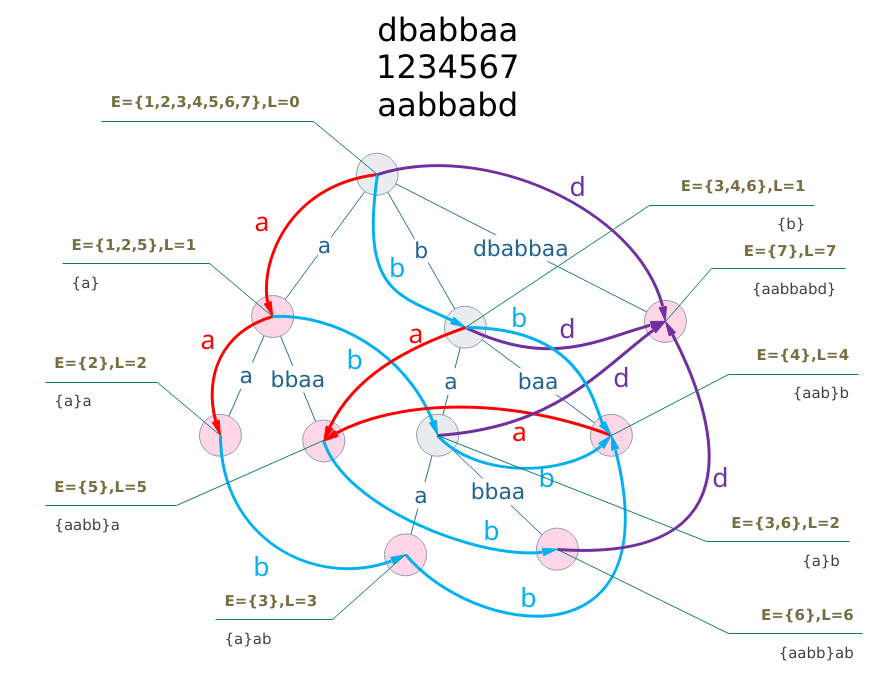
\includegraphics[width=0.8\linewidth]{assets/sam.png}
\end{center}


\end{document}
